\documentclass{article}\usepackage[]{graphicx}\usepackage[]{xcolor}
% maxwidth is the original width if it is less than linewidth
% otherwise use linewidth (to make sure the graphics do not exceed the margin)
\makeatletter
\def\maxwidth{ %
  \ifdim\Gin@nat@width>\linewidth
    \linewidth
  \else
    \Gin@nat@width
  \fi
}
\makeatother

\definecolor{fgcolor}{rgb}{0.345, 0.345, 0.345}
\newcommand{\hlnum}[1]{\textcolor[rgb]{0.686,0.059,0.569}{#1}}%
\newcommand{\hlsng}[1]{\textcolor[rgb]{0.192,0.494,0.8}{#1}}%
\newcommand{\hlcom}[1]{\textcolor[rgb]{0.678,0.584,0.686}{\textit{#1}}}%
\newcommand{\hlopt}[1]{\textcolor[rgb]{0,0,0}{#1}}%
\newcommand{\hldef}[1]{\textcolor[rgb]{0.345,0.345,0.345}{#1}}%
\newcommand{\hlkwa}[1]{\textcolor[rgb]{0.161,0.373,0.58}{\textbf{#1}}}%
\newcommand{\hlkwb}[1]{\textcolor[rgb]{0.69,0.353,0.396}{#1}}%
\newcommand{\hlkwc}[1]{\textcolor[rgb]{0.333,0.667,0.333}{#1}}%
\newcommand{\hlkwd}[1]{\textcolor[rgb]{0.737,0.353,0.396}{\textbf{#1}}}%
\let\hlipl\hlkwb

\usepackage{framed}
\makeatletter
\newenvironment{kframe}{%
 \def\at@end@of@kframe{}%
 \ifinner\ifhmode%
  \def\at@end@of@kframe{\end{minipage}}%
  \begin{minipage}{\columnwidth}%
 \fi\fi%
 \def\FrameCommand##1{\hskip\@totalleftmargin \hskip-\fboxsep
 \colorbox{shadecolor}{##1}\hskip-\fboxsep
     % There is no \\@totalrightmargin, so:
     \hskip-\linewidth \hskip-\@totalleftmargin \hskip\columnwidth}%
 \MakeFramed {\advance\hsize-\width
   \@totalleftmargin\z@ \linewidth\hsize
   \@setminipage}}%
 {\par\unskip\endMakeFramed%
 \at@end@of@kframe}
\makeatother

\definecolor{shadecolor}{rgb}{.97, .97, .97}
\definecolor{messagecolor}{rgb}{0, 0, 0}
\definecolor{warningcolor}{rgb}{1, 0, 1}
\definecolor{errorcolor}{rgb}{1, 0, 0}
\newenvironment{knitrout}{}{} % an empty environment to be redefined in TeX

\usepackage{alltt}
\usepackage{amsmath} %This allows me to use the align functionality.
                     %If you find yourself trying to replicate
                     %something you found online, ensure you're
                     %loading the necessary packages!
\usepackage{amsfonts}%Math font
\usepackage{graphicx}%For including graphics
\usepackage{hyperref}%For Hyperlinks
\usepackage[shortlabels]{enumitem}% For enumerated lists with labels specified
                                  % We had to run tlmgr_install("enumitem") in R
\hypersetup{colorlinks = true,citecolor=black} %set citations to have black (not green) color
\usepackage{natbib}        %For the bibliography
\setlength{\bibsep}{0pt plus 0.3ex}
\bibliographystyle{apalike}%For the bibliography
\usepackage[margin=0.50in]{geometry}
\usepackage{float}
\usepackage{multicol}

%fix for figures
\usepackage{caption}
\newenvironment{Figure}
  {\par\medskip\noindent\minipage{\linewidth}}
  {\endminipage\par\medskip}
\IfFileExists{upquote.sty}{\usepackage{upquote}}{}
\begin{document}

\vspace{-1in}
\title{Lab 7/8 -- MATH 240 -- Computational Statistics}

\author{
  Jake Schneider \\
  Colgate University  \\
  Mathematics  \\
  {\tt jdschneider@colgate.edu}
}

\date{}

\maketitle

\begin{multicols}{2}
\begin{abstract}
This lab report focuses on understanding and applying the beta distribution. We examined its theoretical properties by computing the mean, variance, skewness and kurtosis across four parameter settings. Using both numerical integration and simulated data, we verified the population moments and explored how sample statistics converge to their theoretical values. We applied these concepts to real world data by modeling country level death rates. We estimated the distribution parameters using both Method of Moments (MOM) and Maximum Likelihood Estimation (MLE). Overall this lab highlights the flexibility of the beta distribution and its usefulness in modeling bounded, proportion based data. 
\end{abstract}

\noindent \textbf{Keywords:} Beta Distribution, Point Estimation, Simulation

\section{Introduction to Beta Distribution}
The beta distribution is a flexible, continuous probability distribution used to model a random variable X on the interval [0,1] or (0,1) in terms of two positive parameters, alpha and beta. These two parameters control the shape of the distribution. The properties of the beta distribution make it useful for modeling proportions, probabilities or rates due to its ability to take on a wide range of forms.

\section{Density Functions and Parameters}
The beta distribution's probability density function is defined as:
\[
f(x \mid \alpha, \beta) = \frac{\Gamma(\alpha + \beta)}{\Gamma(\alpha)\Gamma(\beta)} x^{\alpha - 1}(1 - x)^{\beta - 1}I(x \in [0,1])
\]

In our function $\alpha$ and $\beta$ are the shape parameters and $\Gamma$ is the gamma function. This allows the beta distribution to be remarkably flexible with regards to its shape; it can be left-skewed, right skewed or symmetric depending on the value of the parameters that define its shape which we can see if we look to Figure \ref{plot1} which illustrates how the shape can change across the four different parameter combinations. Summary statistics for each of these cases are presented in Table \ref{table2}, offering a clearer understanding of how the distribution behaves under various conditions, which we also summarize more generally below. 
\begin{itemize}
\item $\alpha$$>$1, $\beta$$>$1: The distribution is uni modal and resembles a bell curve.
\item $\alpha$$<$1, $\beta$$<$1: The distribution is U-shaped, with a higher density near 0 and 1.
\item $\alpha$=$\beta$=1: The distribution simplifies to a uniform distribution over [0,1].
\item $\alpha$$>$1, $\beta$$<$1: The distribution skews towards 1.
\item $\alpha$$<$1, $\beta$$>$1: The distribution skews towards 0.
\end{itemize}


\section{Properties}
These are several of the key properties for the beta distribution.
\begin{align}
\mathbb{E}(X) &= \frac{\alpha}{\alpha + \beta} && \tag{Mean} \\
\text{Var}(X) &= \frac{\alpha \beta}{(\alpha + \beta)^2(\alpha + \beta + 1)} && \tag{Variance}  \\
\text{Skew}(X) &= \frac{2(\beta - \alpha)\sqrt{\alpha + \beta + 1}}{(\alpha + \beta + 2)\sqrt{\alpha \beta}} && \tag{Skewness} \\
\text{Kurt}(X) &= 6 \cdot \frac{(\alpha - \beta)^2(\alpha + \beta + 1) - \alpha \beta (\alpha + \beta + 2)}{\alpha \beta (\alpha + \beta + 2)(\alpha + \beta + 3)} && \tag{Excess Kurtosis}
\end{align}

These formulas are used to compute the true values of the mean, variance, skewness, and excess kurtosis for our various parameter combinations. To verify them numerically, we created a R function called \verb|beta.moment()|, that computes both centered and uncentered arguments using numerical integration. We can see compare our numerical summaries in Table \ref{table2} to our theoretical summaries in Table \ref{table1} to see they are indeed very close.

In addition, by generating a large number of samples from a know beta distribution with parameters $\alpha$=2 and $\beta$=5 we demonstrated that the sample based estimates of these statistics being to converge to their true population-level statistics which we can see in Figure \ref{plot2}, which was done using the \texttt{cumstats} package \citep{cumstats}. This convergence demonstrates the Weak Law of Large Numbers. Furthermore, when we modeled the sampling distribution of these statistics we see that in Figure \ref{plot3} that our resulting distributions are narrow and symmetric. This would indicate to us that our estimates were not only accurate but also precise. Together, these results support the reliability of using sample based summaries to approximate population characteristics for the Beta Distribution.


\section{Estimators}
When applying the beta distribution, estimating the parameters $\alpha$ and $\beta$ is critical for real world application.
The two methods that we can use for estimating these parameters are:
\begin{itemize}
\item Method of Moments (MOM): This method equates the first k sample moments to the first k population moments of the Beta Distribution to solve for $\alpha$ and $\beta$.
\item Maximum Likelihood Estimation (MLE): This approach creates a likelihood function based on the distributions probability density function (PDF) and identifies the parameter values that maximize the likelihood of observing the given data.
\end{itemize}


To assess the performance of our estimators we can compare the estimates using bias, precision and mean squared error (MSE). Bias measures the average deviation from the true parameter value, precision reflects the consistency of the estimates, and MSE captures the overall error by combining both bias and variance. These three metrics provide insight into how well each method estimates the underlying parameters of the distribution. Given a vector of estimates \texttt{theta.hats} and a true value of \texttt{theta}, these quantities can be computed as follows. 
\[
\text{Bias} = \mathbb{E}(\hat{\theta}) - \theta
\]
\[
\text{Precision} = \frac{1}{\text{Var}(\hat{\theta})}
\]
\[
\text{MSE} = \text{Var}(\hat{\theta}) + \left( \mathbb{E}(\hat{\theta}) - \theta \right)^2
\]


\section{Example: Modeling Death Rates}
To apply the beta distribution, Fatih (\citeyear{fatih2022determinants}) suggest that country death rates can be modeled by the beta distribution. We collected data from the World Bank on country's death rates in 2022. Since death rates are naturally bounded between 0 and 1 when being expressed as proportions the beta distribution would be a good distribution for this data.  

\subsection{Collecting Data and Estimating Parameters}
The data we collected reported death rates per 1000 citizen, and the support for the beta distribution is (0,1), so we need to convert this rate into a proportion to ensure they fall are within the support so we divide each value by 1000. To clean the data we selected the country name, code and year 2022. Once the data was collected and cleaned we then estimated the parameters $\alpha$ and $\beta$ using the both the MOM and MLE techniques. For the MOM technique we used the \texttt{nleqslv} package \citep{nleqslv} and the function \verb|nleqslv()|. As for the MLE method we used the \verb|optim()| function to maximize the negative log-likelihood function. 

To evaluate the the performance of each method, we simulated 1000 iterations using a \verb|for()| loop with $\alpha$=8 and $\beta$=950 and used \texttt{set.seed(7272+i)}. This generated 1000 estimates for $\alpha$ and $\beta$ for both the Method of Moments and Maximum Likelihood Estimation. We can see the distribution of our estimates if we look to Figure \ref{plot4}. We also created table to summarize the accuracy and precision of our estimates to help us determine which method performs better, as shown in Table \ref{table3}.

\subsection{Results}
The simulation results collected show a distinct difference between the MOM and MLE estimators. The distribution of MLE estimators for both $\alpha$ and $\beta$ are more concentrated around the true parameter values compared to the MOM estimates. This is visible in our density plots in Figure \ref{plot4} which shows a more narrow and symmetric curve for both parameters of the MLE function. The table below also shows a numerical summary of the performance for each of the techniques. 
\begin{center}
\small
\captionof{table}{Summary Statistics Estimator Distribution}
\label{table3}
\begin{tabular}{rllrrr}
  \hline
 & Method & Parameter & Bias & Precision & MSE \\ 
  \hline
1 & MOM & Alpha & 0.08 & 1.83 & 0.55 \\ 
2 & MOM & Beta & 10.57 & 0.00 & 8303.00 \\ 
3 & MLE & Alpha & 0.07 & 2.13 & 0.47 \\ 
4 & MLE & Beta & 9.18 & 0.00 & 7118.73 \\ 
  \hline
\end{tabular}
\end{center}

We see in our table that MLE outperformed MOM with a lower bias, higher precision and smaller MSE for all of the parameters, that is we would opt to use the MLE technique as the most accurate method to estimate our parameters. 

\subsection{Discussion}
This examples demonstrates how the beta distribution can be applied to real world examples of proportions that are naturally bounded between 0 and 1. Through both theoretical and applied analysis, we gained insight into the flexibility and the behavior given different parameters. 

Both MOM and MLE offered estimates that would we could have used for our distributions parameters. We saw that MOM is simpler to implement and easier to interpret, however it was sightly more varied and less accurate compared to MLE. Once we have successful fitted a beta distribution to real data, we can now start to as some questions about the data. For example we may ask, what is the probability that a country's death rate exceeds a certain percentage? Or, if the World Health Organization wanted to allocate more resources to the worst 10\% of countries what would the death rate cutoff be? While these are not questions that we will answer in this lab it is important to consider the useful applications that our information may be able to provide to help us solve real world problems. To answer these question to the best of our ability, it is essential to establish a strong statistical foundation that supports accurate and reliable results.


%%%%%%%%%%%%%%%%%%%%%%%%%%%%%%%%%%%%%%%%%%%%%%%%%%%%%%%%%%%%%%%%%%%%%%%%%%%%%%%%
% Bibliography
%%%%%%%%%%%%%%%%%%%%%%%%%%%%%%%%%%%%%%%%%%%%%%%%%%%%%%%%%%%%%%%%%%%%%%%%%%%%%%%%
\vspace{1em}


\begin{tiny}
\bibliography{bib}
\end{tiny}
\end{multicols}

%%%%%%%%%%%%%%%%%%%%%%%%%%%%%%%%%%%%%%%%%%%%%%%%%%%%%%%%%%%%%%%%%%%%%%%%%%%%%%%%
% Appendix
%%%%%%%%%%%%%%%%%%%%%%%%%%%%%%%%%%%%%%%%%%%%%%%%%%%%%%%%%%%%%%%%%%%%%%%%%%%%%%%%
\newpage
\onecolumn
\section{Appendix}

\begin{figure}[H]
  \begin{center}
  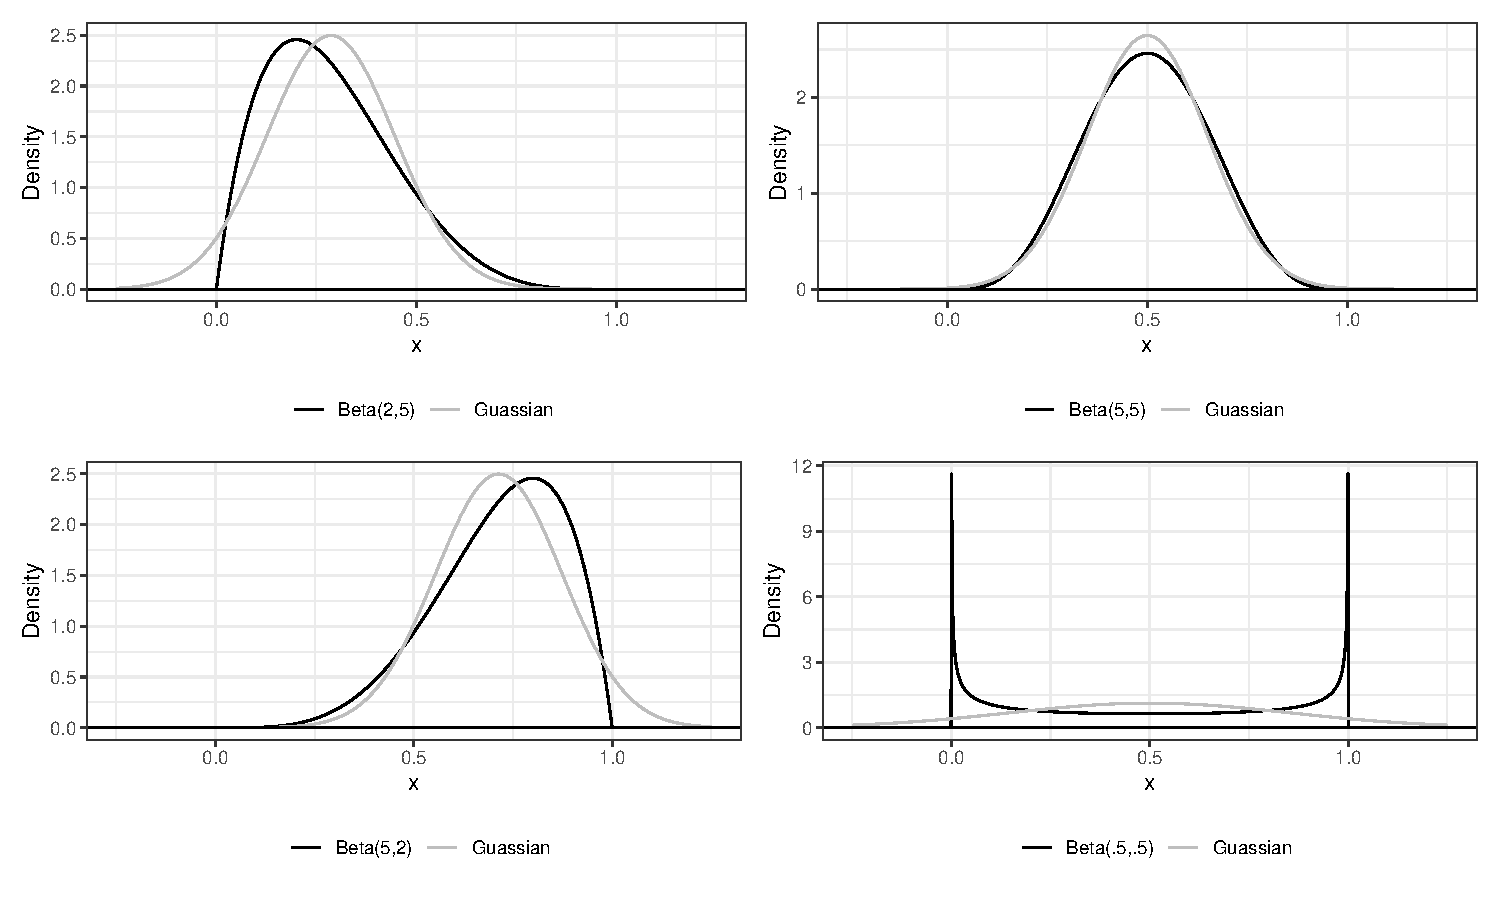
\includegraphics[width=\textwidth]{varying.beta.distributions.pdf}
  \caption{4 Beta Distribution Cases}
  \label{plot1}
  \end{center}
\end{figure}

\begin{table}[ht]
\centering
\caption{Population Level Summary Statistics Of 4 Beta Distribution Parameters}
\label{table1}
\begin{tabular}{rrrrrrr}
  \hline
 & Alpha & Beta & Mean & Variance & Skewness & Excess Kurtosis \\ 
  \hline
1 & 2.00 & 5.00 & 0.29 & 0.03 & 0.60 & -0.12 \\ 
  2 & 5.00 & 5.00 & 0.50 & 0.02 & 0.00 & -0.46 \\ 
  3 & 5.00 & 2.00 & 0.71 & 0.03 & -0.60 & -0.12 \\ 
  4 & 0.50 & 0.50 & 0.50 & 0.12 & 0.00 & -1.50 \\ 
   \hline
\end{tabular}
\end{table}

\begin{table}[ht]
\centering
\caption{Numeical Summary Statistics of 4 Beta Dsitribution Parameters}
\label{table2}
\begin{tabular}{rrrrrrr}
  \hline
 & Alpha & Beta & Sample Mean & Sample Variance & Sample Skewness & Sample Excess Kurtosis \\ 
  \hline
1 & 2.00 & 5.00 & 0.29 & 0.03 & 0.57 & -0.23 \\ 
  2 & 5.00 & 5.00 & 0.50 & 0.02 & -0.06 & -0.58 \\ 
  3 & 5.00 & 2.00 & 0.71 & 0.03 & -0.57 & -0.23 \\ 
  4 & 0.50 & 0.50 & 0.51 & 0.13 & -0.02 & -1.51 \\ 
   \hline
\end{tabular}
\end{table}

\begin{figure}[ht]
  \begin{center}
  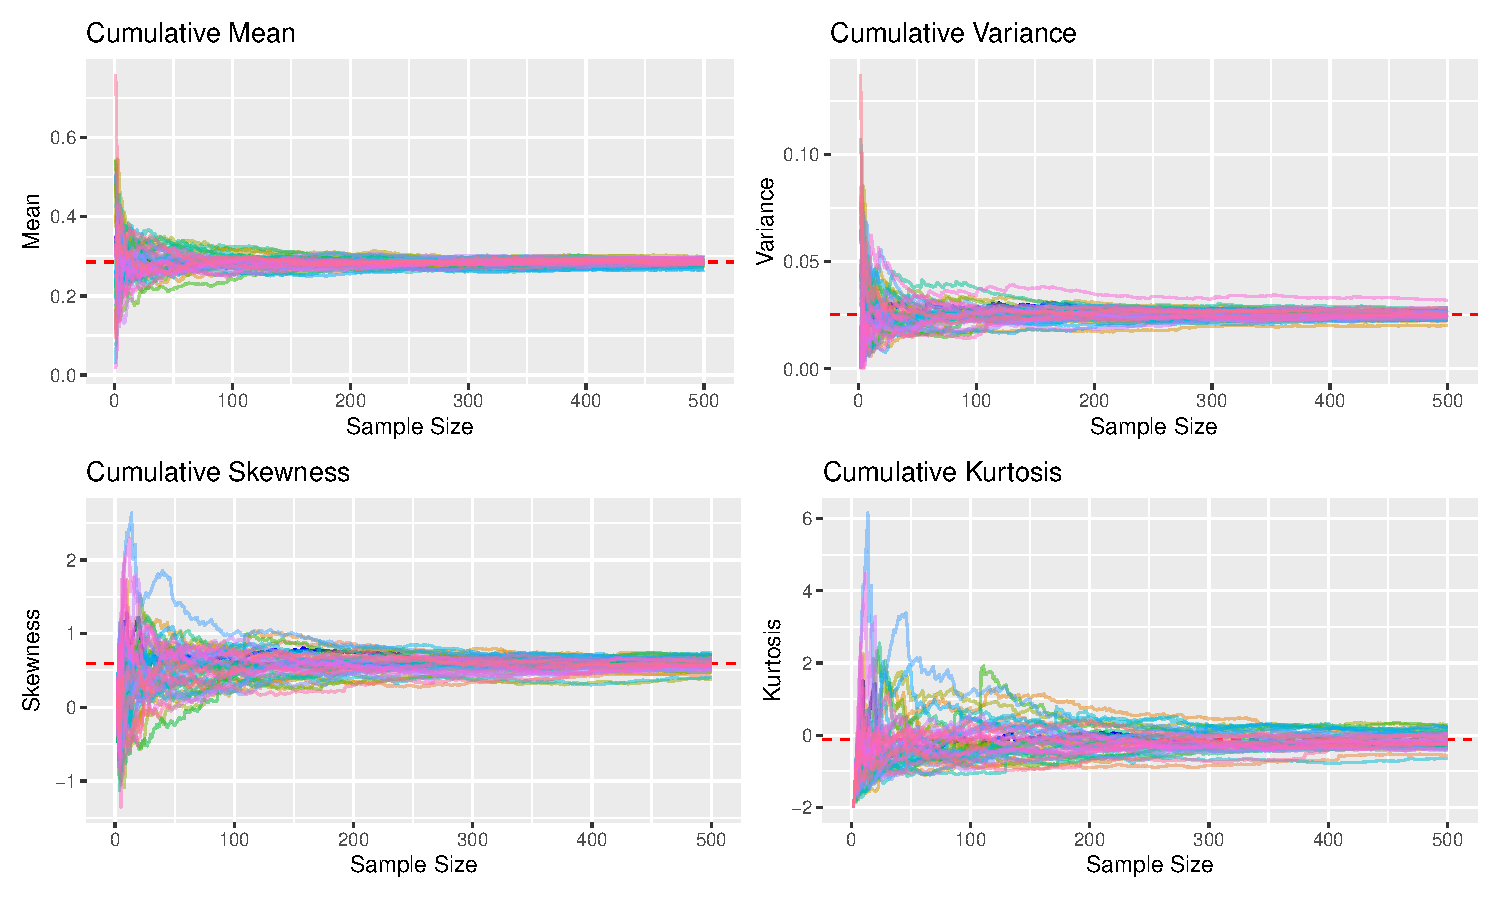
\includegraphics[width=\textwidth]{convergence.plots.pdf}
  \caption{$\alpha$=2 and $\beta$=5 Convergence Simulation}
  \label{plot2}
  \end{center}
\end{figure}

\begin{figure}[ht]
  \begin{center}
  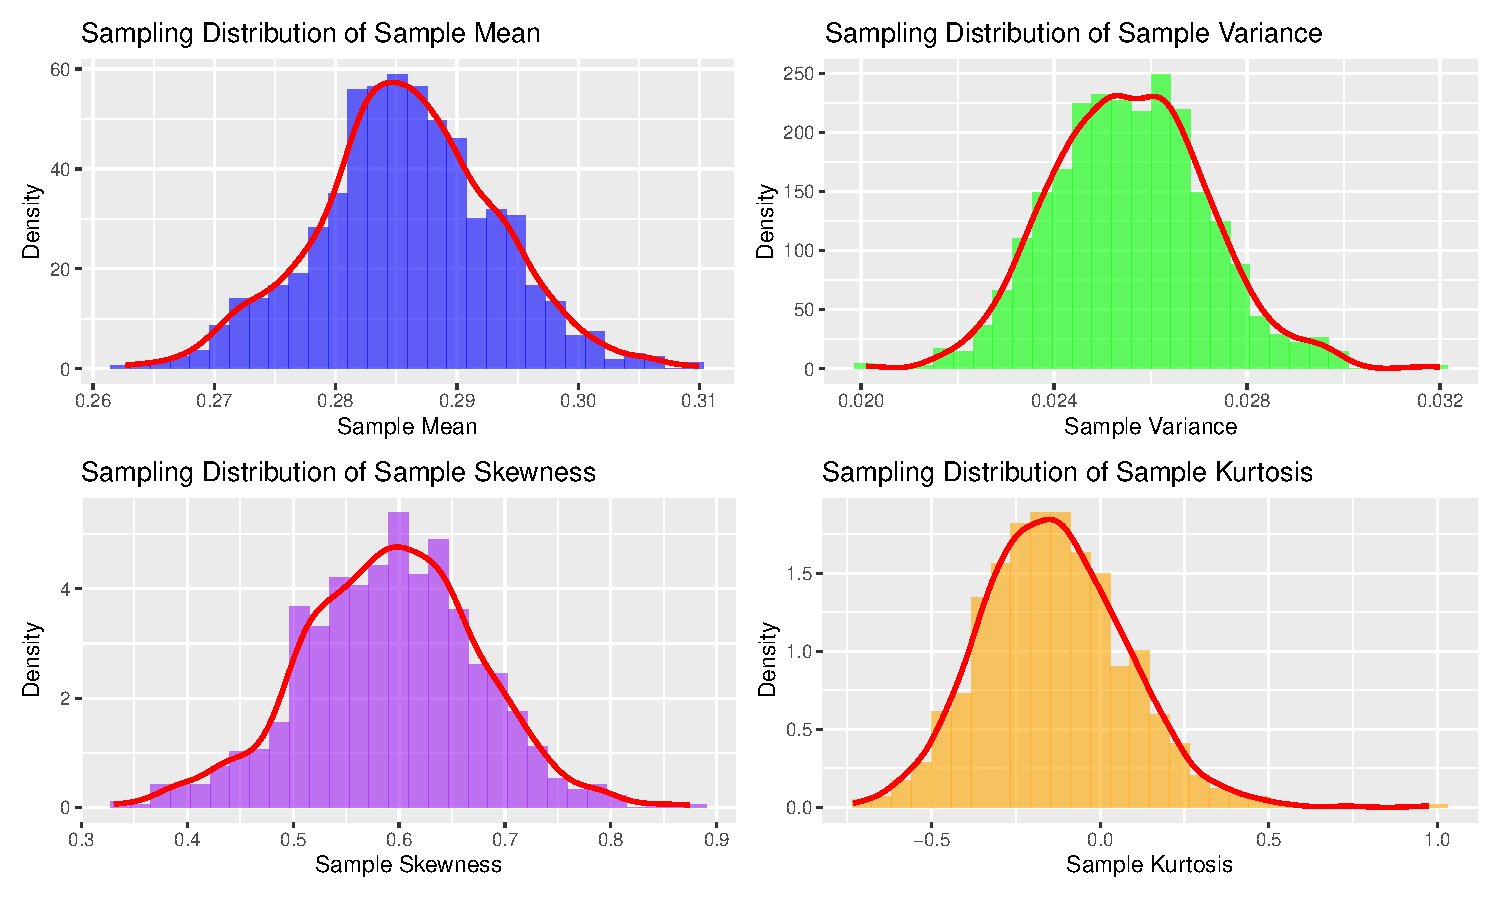
\includegraphics[width=\textwidth]{variation.distributions.pdf}
  \caption{$\alpha$=2 and $\beta$=5 Sampling Distribution Variation}
  \label{plot3}
  \end{center}
\end{figure}

\begin{figure}[ht]
  \begin{center}
  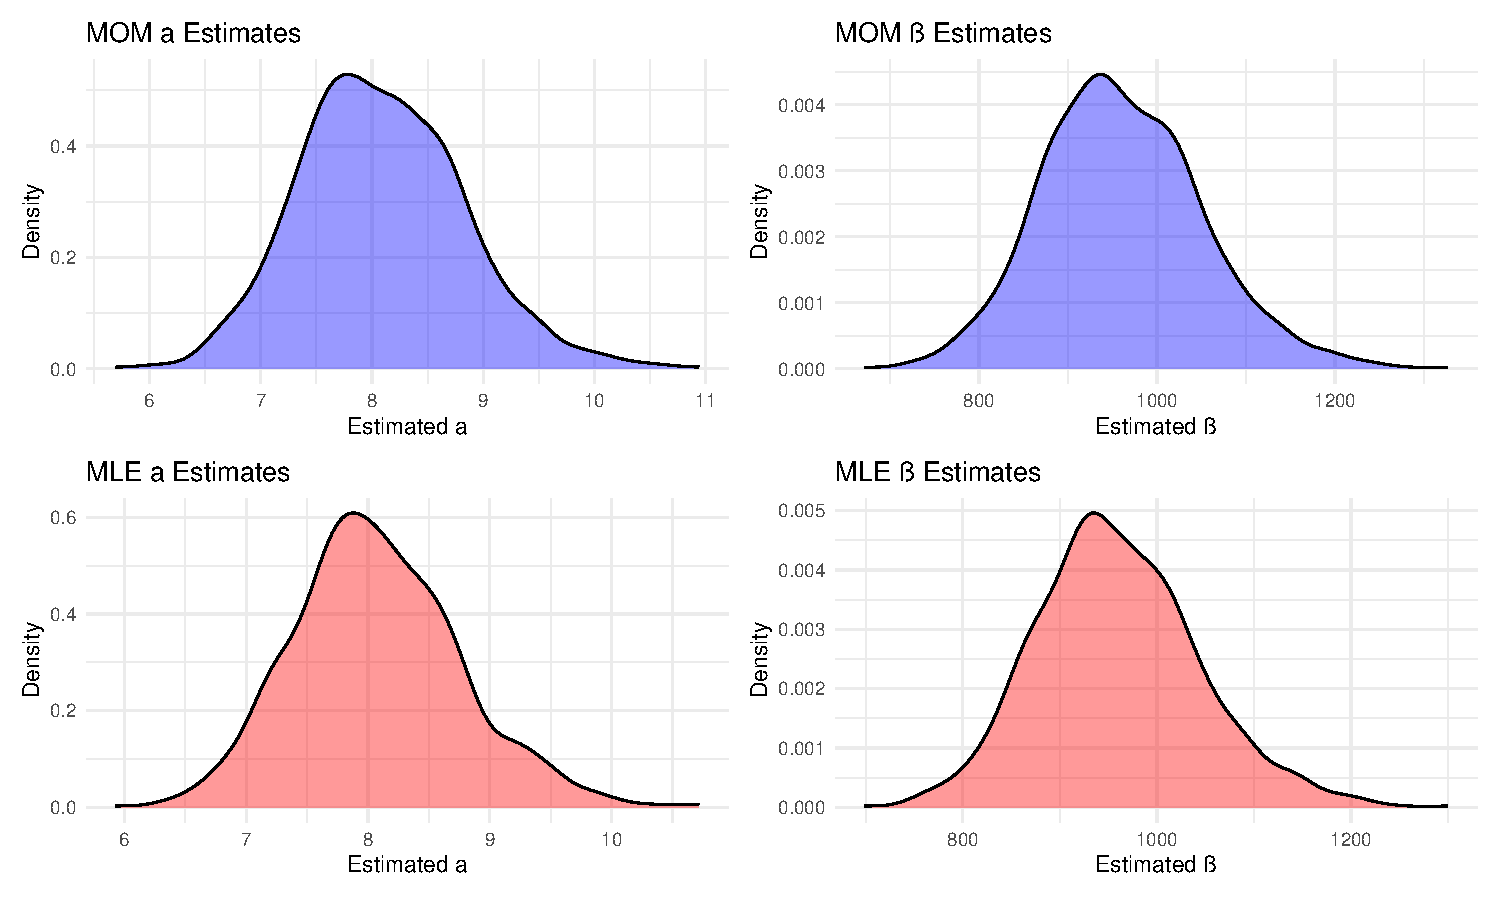
\includegraphics[width=\textwidth]{estimator.plot.pdf}
  \caption{Estimator Distribution}
  \label{plot4}
  \end{center}
\end{figure}


\end{document}
